\chapter{Background}
\section{Problem Context}
$Problem Context:
If your project involves significant work on a non-computing topic that is likely to be unfamiliar to most readers (e.g. linguistics, fluid dynamics) you should describe the important principles, concepts and terminology of that subject area in some detail. You will have had to learn these yourself in getting to grips with this unfamiliar topic and you should summarize what you learnt to enable the reader to understand your subsequent discussion on your project work and how this relates to the wider topic area.
$



The main focus of this project is to create a network degradation tool that can be used to simulate imperfect network conditions. To understand the goal better it is important to know what criteria reduce network quality.

Latency, packet loss and bandwidth are the main factors that distinguish between good and bad internet connections. Latency is the delay between sending a message and seeing its result. Packet loss is the percentage of packets that are lost in transmission, the higher the percentage, the more effect it has on the speed and stability of the network. Bandwidth, is the measure of how many bits/bytes are being transferred per second, the larger the bandwidth the more data can be transferred in less time, thus making the overall connection faster. A combination of favourable values from these criteria defines a good network connection. One way to visualise the throughput of a network connection is a download and upload and speed test, the result of these is measured in Mbps and can be used to quickly compare the speed of two connections, this will be used later to briefly show the degradation.

It is also necessary to mention the protocols that are to be used in the network simulation section. TCP \citep{TCP} and UDP \citep{UDP} are the transport layer protocols up for discussion. 

Other small signs of poor network conditions is Jitter and Error rate. Jitter is simply the variance in packet delays, this is normally a issue that exists in large packet switched networks, this is however not an issue in TCP/IP based communications because TCP protocol deals with these issues. However, VoIP (Voice over IP) that uses UDP as its transport level protocol is visibly degraded by heavy jitter. Error rate is the number of bit errors that have occurred in a data stream over a period of time. This can again effect UDP based communications heavily but the TCP protocol deals with these issues so remains relatively unaffected.

\comments{Talk about how TCP deals with jitter?}
\comments{Talk more about Packet Loss/Latency/Packet Loss maybe even about smaller signs of bad connection quality?}

\subsection{Protocols}
\subsubsection{Transport Control Protocol (TCP)}
TCP's main design choices are centred around reliability, where it has a few techniques designed to make sure packets arrive correctly. The connection begins by being initiated with a series of signals where they are abbreviated as ACK (Acknowledgement) and SYN (Synchronise). The first computer begins by sending an packets with the SYN flag set, this starts the synchronization process. Then once the target computer receives this SYN packet it sends back and ACK for that SYN and its own SYN to the initiating computer, so an ACK + SYN packet, where finally the initial computer sends back an ACK packet for the previous SYN packet, this connection has now been initiated and the communication channel has been set up. This process is known as a `handshake'.

For TCP to remain reliable it needs to maintain data on the status of a connection, where a connection is uniquely identified by the pair of sockets that define its two sides. The information retained contains, sequence number and window sizes where these values are used to calculate the expected next packet to therefore calculate if a packet has been retransmitted or if a packet has been send out of its order.

\comments{Add image displaying this process}



% How does TCP deal with errors?
% - Numbers packets
% - Send Ackowlegements per 
%	- If ACK isn't recieved in the timeout period the packet is reset
% - Resending of missing packets
%		- Why Packet loss isn't terrible on performance

\comments{More about TCP, talk about how it detects a missing packet etc}

\subsubsection{User Data Protocol (UDP)}
UDP is by design the opposite of TCP and often you'll find the two protocols compared. UDP is often referred to as ``fire and forget" \citep{kempf2011thoughts} this is a short way of describing how UDP deals with packets. When a packet is to be sent UDP sends the packet and moves onto the next. However, this means aside from the checksum in the UDP header (A checksum can be used to check that the UDP data has been transferred correctly) there is zero error checking for the UDP protocol and results in UDP being considered unreliable in comparison to TCP. This lack of error-checking overhead however, greatly improves the speed of UDP protocols. UDP is not used in situations where communication is vital, but does find itself implemented in examples like voice or video chat because errors in these services are not catastrophic to operation and these imperfections can even go unnoticed. 

\comments{Talk more about UDP, what contained in the header etc}

The tool will be deployed either by having it run on a small custom computer set up to act as a router for the synthetic test network or by jumping between a user and an actual router on a live network. The program will achieve this jumping between a user and the router by utilising a long term vulnerability in the Address Resolution Protocol (ARP) \citep{arp2001}, before this is explained further it is first important to understand the relevant parts of a local network.

\subsubsection{Address Resolution Protocol (ARP)}
Each computer on a Local Area Network (LAN) has an IP assigned to it, this is the identifier on the local network, with this each computers wireless card has a MAC address, a MAC address is a unique identifier for a computer and is used to link up this non-unique local address (IP) to a real computer on a network, this combination of IP address and MAC address allow for the reuse of local IP numbers. The ARP protocol is used to find out what MAC address is associated with a local IP address and visa versa. This is achieved via an entire network broadcast where computers that don't match ignore the ARP request, and the one being requested sends back a reply containing it's MAC address, this is achieved without any authentication. Therefore, this means a program can send out fake custom ARP requests to change specific values in the routers ARP table, meaning a computer running this software can appear as the router to the victim, while also appearing as the victim to the router, thus having all the traffic between the two routed through the attacking computer. 

\comments{Talk more about how a network resolves IP address and why ARP is vuln}
\comments{Need to go deeper into ARP, I really want to show I fully understand what is happening here}

\begin{center}
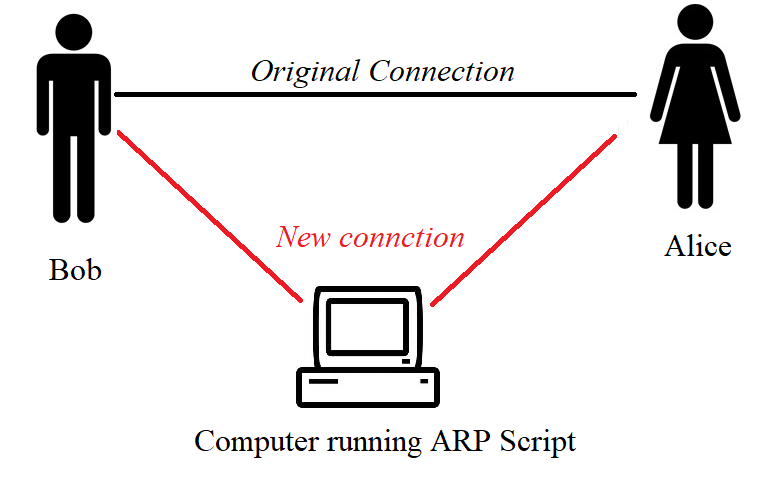
\includegraphics[scale=0.7]{mitm}
	\begin{figure}[h]
		\caption{Photo depicting a MITM attack}
	\end{figure}
\end{center}

\subsubsection{Raspberry Pi}
As mentioned previously the effects will be performed on a custom computer acting as the router, because the network will be set-up to pass all traffic through this router, it will be able to simulate degradation on the entire networks traffic.
The Raspberry Pi \citep{upton2014raspberry} has been decided as the choice for the small custom computer. Originally designed to teach children to code on an inexpensive (less than £30) computer, the Pi has found itself involved in a multitude of uses ranging from NAS (Network Attached Server) to robot controllers. This is useful in this project due to its ease to set-up as a router, this is because of the easy access of low level aspects of the operating system due to it running a based OS. The Raspberry Pi will be run with its default Raspbian OS \citep{pi2014raspbian} that is built upon Debian \citep{murdock1994overview}. This is a optimised OS for the internal ARM CPU that allows the Raspberry Pi to run modern stripped down programs on its very limited hardware, where it will have plenty of power to easily handle traffic as a router.
\comments{Talk more about the structure of the Pi, maybe some tech specs?}

\section{Comparison of Technologies}
$Comparison of Technologies:$
$If there are several possible technologies that could be used in your project work you should present a comparative analysis and critical appraisal of each of these technologies. You should create a subsection for each of the technologies you discuss and title each subsection with the name of the technology it describes (e.g. object-oriented databases, XML ). Within each subsection you should provide an overview of the technology, its key features and its strengths and weaknesses in relation to your project.$

\subsection{Protocol Comparison}
\subsubsection{TCP Based Protocols}
TCP has various protocols built on top of it. One of the most widely used protocols is HTTP/1.1 \citep{HTTP}. HTTP is a structured language used to transfer data worldwide. Its main use is the movement of web based data, this has been chosen as one of the protocols to be used in the test network to simulate live real-world traffic, this is due to the protocols heavy use in the real world. The protocol will be utilised by a web browser that attempts to access a web page, the degradation will therefore be visible through how quickly the web page loads and how responsive the connection seems.

Another protocol based on top of TCP is FTP (File Transfer Protocol) \citep{FTP}, and as the broken down acronym suggests is the protocol used to transfer files across a network. This protocol has been selected also due to its integral use in a live network. It also has a quite intuitive way of representing the speed of a network through a download speed that is easy to understand for most users. The protocol will be tested with dummy files ranging from 1MB to 5GB. This size range was chosen to fully cover the normal spectrum of file size where it roughly ranges from a Word document to high quality video.

\subsubsection{Other TCP Considerations}
SFTP (SSH File Transfer Protocol) \citep{SFTP} was a consideration as a protocol to be used for the demonstration purposes. SFTP effectively is a secure version of FTP (but not to be mixed up with the Simple File Transfer Protocol). This was decided not to be used because of its added features such as authentication security does not fit within the scope of the project, and does not relate to network degradation. 

\comments{More considered protocols}


\subsubsection{UDP Based Protocols}
UDP due to its speed but inherent unreliability, UDP is hugely affected by packet loss. Therefore, the effects on UDP has decided to be visualised by a program that simulates image transfer by assigning an individual UDP packet a number that corresponds to a single pixel, this packet is then sent. Once the server receives the packet, it reads the pixel number stored in the packet and changes that specific pixel to green. This creates a matrix of red (lost) and green(received) pixels. This therefore, gives a simple but effective visualisation of packet loss. 

\begin{center}
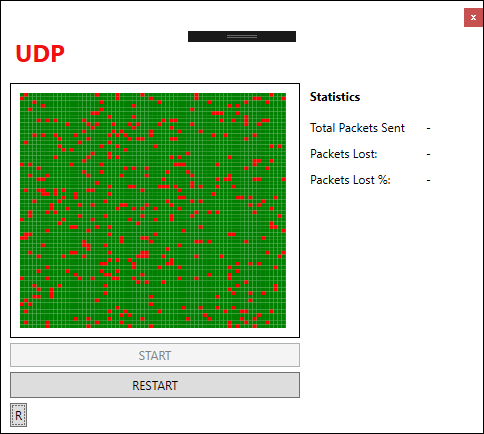
\includegraphics[scale=0.7]{UDP-Demo}
	\begin{figure}[h]
		\caption{Initial draft of the UDP user interface}
	\end{figure}
\end{center}

UDP could have been utilised through real world applications like voice/video chat or an on-line game, but the added complexity to implement these compared to the simpler pixel based approach would've provided no added value to visualising the effects of the degradation on the connection.

\comments{More UDP protocols}
\comments{Different transfer level considerations here}

\subsection{Operating Systems}

\subsubsection{Linux}
Linux is the broad definition of a family of computer operating systems. The defining characteristics of a ``Linux" OS is the free and open source approach and the use of the Linux Kernel. Android for example has the largest market share in the mobile OS market \citep{share2015desktop}, Android utilises the Linux kernel as the centre for its operating system.

Linux was chosen for this project for its open source element that allows easy access to low-level features in the kernel. The section of the kernel that deals with the filtration of packets for uses like firewalls and packet sniffers is referred to as the ``NetFilter". This acts as an API of sorts where packets can be routed to the net-filter queue to await a verdict (accept or drop) before being moved on. This is the basis for the functionality of the program, it will run on the Raspberry Pi and route all packets that enter the box to the queue where the program will perform its effects on the packets. Latency for example is one of the simplest effect to simulate, the packet will be routed into the queue, taken out and stored and the delay between storing and accepting will be the set latency value and therefore simulating the effect of latency on that packet.

\comments{Get deeper into the Netfilter kernal area. Even start talking about other tools like iptables}

\subsubsection{Windows}
Linux was chosen over the other possible alternative; Windows. The Windows OS is distributed as closed source software under proprietary licences meaning to understand what is happening under the hood is far more difficult. The operating system is documented well and there is support for this form of functionality but due to the transparency of Linux, Linux was chosen as a more suitable alternative.   

\comments{Talk more about windows}

\section{Alternative Solutions}
$Alternative Solutions:$
$If others have produced solutions or addressed similar problems to those addressed by your project you should describe those alternative solutions here. Similarly, if several possible approaches suggest themselves as ways of solving the problems inherent in your project you should discuss those here. You should provide a comparative analysis and critical appraisal of each alternative solution approach or existing solution, identifying their key features and their strengths and weaknesses in relation to your project.$

\comments{For all the solutions I need to be much more critical of the positives and negatives}

\subsection{clumsy}
A more modern application of network degradation is clumsy 0.2 \footnote{\url{http://jagt.github.io/clumsy/index.html}}. It provides various options (that can run in parallel) that effect network conditions. 

\begin{center}
	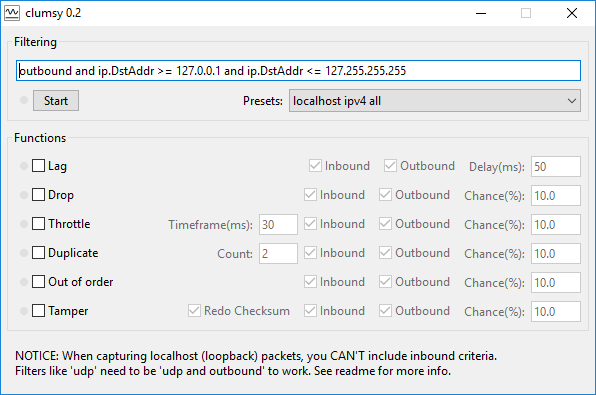
\includegraphics[scale=0.5]{clumsy}
	\begin{figure}[h]
		\caption{Main UI of clumsy}
	\end{figure}
\end{center}

The tool provides a way to affect network conditions. It solves issues involved with simulating harsh network conditions on a network. It does allow for filtering and has a couple of filter pre-sets, it however doesn't provide options to simulate live traffic and options to capture or visualise traffic is not part of the main package.

This tool provides and easy to use and simple tool, but only affects the traffic on the local machine, this is good for testing tools in the development stage of an application but cannot be used to simulate degradation across a simulated network.

\subsection{TMNetSim}
TMNetSim \footnote{\url{http://www.tmurgent.com/appv/en/87-tools/performance-tools/177-tmnetsim-quick-and-easy-network-simulation-tool}} is another tool that covers aspects of this project. Unlike clumsy TMNetSim is designed to provide degradation that expands over the network. However, to achieve this it has to be set-up on every machine, this is clunky and time consuming. The project being developed can negate this lengthy set-up with the intended inclusion of the ARP Spoofing. Further criticism relates to the ease of use of this application, it has a large number of controls on it's interface and will involve a larger learning curve to master compared to other simpler tools, this however might be the bi-product of more functionality; increased complexity.

This tool includes very complex ways of simulating realistic degradation with Gausian and ``Normal" delay modes, that attempt to provide more accurate representations of real-world delays. This is a great feature that could drastically improve the accuracy in simulating degradation and will need to be considered as an extra inclusion into this project.

$Comparison of Algotithms$
$There may be a number of different algorithms which could be applied to the central problems in your project and you have had to choose which of these algorithms are the most appropriate for your implementation. If this is the case then you should provide a comparative analysis and critical appraisal of each of the potentially applicable algorithms, highlighting their key features and their strengths and weaknesses in relation to your project.$

$Process and Methodology$
$If your project is concerned with improving, implementing or evaluating a particular technical process or method of working you should discuss these in detail. We are not expecting you to describe what software development methodology you are following in implementing your project and you certainly do not need to regurgitate textbook descriptions of the Waterfall method here as everyone already knows that model well.$

$This is a narrative description of the general context within which your project fits. Depending on your particular project characteristics, you are required to include discussion of any or all of the following – previous related work; the work or objectives of a client; the essential principles of systems or techniques you are using.$
$All this narrative should be properly referenced to source material citations. Remember that a high class project will refer to background sources beyond just those on the Web. $

$In writing this section you should pay close attention to your audience and their prior knowledge of the subject(s) that you are discussing. You should assume that your reader is a student who has just completed the second year of your degree programme and can therefore assume that the reader is familiar with all topics taught up to the end of the second year. Anything that is needed to understand your project and its context but which has not been taught by the end of the second year of your degree should be discussed in this background section. $

$This section may include one or more of the following subsections. It is difficult to give prescriptive guidance on which subsections you should include as this depends on the nature of the project you are undertaking – you should discuss this with your supervisor.$